\documentclass{article}

\def\titre{Session 1: Prise en main de l'environnement numérique de l'université}

\usepackage[a4paper,left=20mm,right=20mm,top=25mm,bottom=40mm]{geometry}
\usepackage{enumitem}
\setlist{partopsep=0pt,topsep=1ex}
\usepackage{pifont,euscript}
\usepackage{rotating}
\usepackage{tabu}
\usepackage[usenames,dvipsnames,svgnames]{xcolor}
\usepackage{comment}
\usepackage{colortbl}
\usepackage{titling}
\usepackage{multicol}
\usepackage[french]{babel}
\usepackage{mdframed}
\usepackage{textcomp}
\usepackage{listings}
\lstloadlanguages{Python}

\setlength{\droptitle}{-1.5cm}
\pretitle{\begin{center}\LARGE\sffamily\bfseries}
\posttitle{\par\end{center}\vskip -.5cm}
\preauthor{}
\postauthor{}
\predate{}
\postdate{}

\definecolor{UGEBlue}{RGB}{47,42,133}
\definecolor{vert}{RGB}{78,100,26}
\definecolor{violet}{RGB}{130,25,111}
\definecolor{orange}{RGB}{234,91,12}
\definecolor{rouge}{RGB}{230,56,18}
\definecolor{beige}{RGB}{242,238,231}
\definecolor{bleu}{RGB}{0,74,155}
\definecolor{gris}{RGB}{100,100,100}
\definecolor{commentColor}{rgb}{0.38,0.63,0.69}
\definecolor{stringColor}{rgb}{0.25,0.44,0.63}
\definecolor{typeColor}{rgb}{0.56,0.13,0.00}
\definecolor{keywordColor}{rgb}{0.00,0.44,0.13}
\definecolor{digitColor}{rgb}{0.25,0.63,0.44}

\lstset{ %
  backgroundcolor=\color{white},
  basicstyle=\ttfamily,
  breaklines=true,
  captionpos=b,
  commentstyle={\bfseries\itshape\color{commentColor}},
  escapeinside={\%*}{*)},
  keywordstyle=\color{keywordColor},
  stringstyle=\color{stringColor},
  numbers=left,
  stepnumber=1,
  numberstyle=\scriptsize,
  numbersep=10pt,
  language=Python,
  upquote=true
}
\lstset{%
  literate=%
    {é}{{\'e}}1
    {è}{{\`e}}1
    {ê}{{\^e}}1
    {ë}{{\"e}}1
    {à}{{\`a}}1
    {â}{{\^a}}1
    {ä}{{\"a}}1
    {î}{{\^i}}1
    {ï}{{\"i}}1
    {ù}{{\`u}}1
    {û}{{\^u}}1
    {ü}{{\"u}}1
    {ô}{{\^o}}1
    {ö}{{\"o}}1
    {ç}{{\c c}}1
    {œ}{{\oe{}}}1
    {0}{{{{\color{digitColor}0}}}}1
    {1}{{{{\color{digitColor}1}}}}1
    {2}{{{{\color{digitColor}2}}}}1
    {3}{{{{\color{digitColor}3}}}}1
    {4}{{{{\color{digitColor}4}}}}1
    {5}{{{{\color{digitColor}5}}}}1
    {6}{{{{\color{digitColor}6}}}}1
    {7}{{{{\color{digitColor}7}}}}1
    {8}{{{{\color{digitColor}8}}}}1
    {9}{{{{\color{digitColor}9}}}}1
    {.0}{{{{\color{digitColor}.0}}}}2
    {.1}{{{{\color{digitColor}.1}}}}2
    {.2}{{{{\color{digitColor}.2}}}}2
    {.3}{{{{\color{digitColor}.3}}}}2
    {.4}{{{{\color{digitColor}.4}}}}2
    {.5}{{{{\color{digitColor}.5}}}}2
    {.6}{{{{\color{digitColor}.6}}}}2
    {.7}{{{{\color{digitColor}.7}}}}2
    {.8}{{{{\color{digitColor}.8}}}}2
    {.9}{{{{\color{digitColor}.9}}}}2
    {'h}{{{{\color{digitColor}'h}}}}2
}
\lstset{%
  emph={int,char,void,float,double},
  emphstyle=\color{typeColor}
}

\usepackage{lmodern}
\usepackage{amssymb,amsmath}
\usepackage{ifxetex,ifluatex}
\usepackage[T1]{fontenc}
\usepackage[utf8]{inputenc}
\usepackage{upquote}

\usepackage[unicode=true]{hyperref}
\hypersetup{breaklinks=true,
%            bookmarks=true,
            pdfauthor={},
            pdftitle={\titre},
            colorlinks=true,
            citecolor=blue,
            urlcolor=blue,
            linkcolor=magenta,
            pdfborder={0 0 0}}
\urlstyle{same}  % don't use monospace font for urls
\usepackage{tikz}
\usetikzlibrary{quotes}
\usetikzlibrary{arrows,positioning} 

\tikzstyle{val}=[rectangle,draw]
\tikzstyle{var}=[rectangle,rounded corners=1.5ex,draw,bleu,minimum size=3ex]
\tikzstyle{aff}=[->,thick]
\tikzset{
  every node/.style={font=\footnotesize},
  instr/.style={rectangle,draw=black!70},
  test/.style={rectangle,rounded corners,draw=bleu!70,text=bleu},
  every edge/.style={>=stealth,semithick,bend angle=45,draw,->},
  every edge quotes/.style={inner sep=.5em,font=\scriptsize,color=orange},
  vrai/.style={left,"vrai"},
  faux/.style={right,"faux"},
}
\usepackage{color}
\usepackage{fancyvrb}
\setlength{\parindent}{0pt}
\setlength{\parskip}{6pt plus 2pt minus 1pt}
\setlength{\emergencystretch}{3em}  % prevent overfull lines
\providecommand{\tightlist}{%
  \setlength{\itemsep}{0pt}\setlength{\parskip}{0pt}}
\setcounter{secnumdepth}{5}

\usepackage{fancyhdr}
\fancyhead[L]{
\includegraphics[height=1.1cm]{UPEM-IGM-V1_300dpi.png}}
\fancyhead[C]{{
\bf Pré-rentrée informatique\\
Semaine d'intégration du 5 au 9 septembre 2022\\
}
L1 Informatique \& Mathématiques
}
%\fancyhead[R]{
\includegraphics[height=1.3cm]{logo-ligm.png}}
\setlength{\headheight}{50pt}
\renewcommand{\headrulewidth}{1pt}


% cadres informatifs
\newcommand{\but}[1]{%
\hbox{}\noindent%
\fcolorbox{CadetBlue}{white}{%
  \parbox{\dimexpr\linewidth-2\fboxsep-1pt\relax}{%
    \vskip10pt%
    \leftskip10pt\rightskip10pt%
    #1%
    \vskip10pt}}\medskip\thispagestyle{fancy}}


% Environnements d'exercices

\font\manual=manfnt % font used for the METAFONT logo, etc.
\def\barble{{\manual\char1}}
\def\fulltriangleright{{\manual\char120}} %
\def\fulltriangleup{{\manual\char54}} %
\def\fulltriangledown{{\manual\char55}}
\def\littlecube{{\manual\char28}}
\def\prettystar{{\manual\char30}}
\def\littlecircles{{\manual\char36}}
\def\littlelosanges{{\manual\char37}}
\def\littlecloud{{\manual\char38}}
\def\ellipsoid{{\manual\char88}}
\def\zip{{\manual\char121}} % -/\/->
\def\dbendright{{\manual\char126}}
\def\dbendleft{{\manual\char127}}
\def\question{\noindent\llap{\ding{90}\ding{212}}{\kern1pc}}
\newcounter{exo_count}
\def\exoname{Exercice}
\newenvironment{exercice}[1][]%
{\smallbreak\refstepcounter{exo_count}%
\vspace{0.3cm}%
\begin{sloppypar}\noindent{\fulltriangleright\kern 2pt%
\bf\exoname~\arabic{exo_count} : #1} %
}%
{\end{sloppypar}%
}



\newenvironment{correction}{\subsection*{\textcolor{red}{Correction}}}{\medskip}

\def\labelenumi{\arabic{enumi}.}
\def\labelenumii{\alph{enumii}.}

\title{\color{UGEBlue}\titre}
%\date{Semestre 2}
\date{}


\newcommand{\code}[1]{\lstinline{#1}}
\lstnewenvironment{fullcode}{\lstset{xleftmargin=1.4em}}{}
\lstnewenvironment{nonumbercode}{\lstset{numbers=none}}{}


\excludecomment{correction} 
% Commenter la ligne ci-dessus si on souhaite afficher les corrections

\begin{document}
\maketitle

\but{Dans ce TP vous allez:
\begin{itemize}
\item prendre en main le système d'exploitation Linux (Debian) et son gestionnaire de bureau Gnome ;
\item vous familiariser avec l'organisation des données en répertoires et fichiers ;
\item découvrir les services en ligne fournis par l'université ;
\item accéder au discord de la L1 et adopter les bons comportements sociaux;
\item apprendre à utiliser un notebook Jupyter ;
\item être formé aux autres solutions pour utiliser Linux à la maison;
\item vous connecter au WIFI de l'université;
\item Effectuer votre test de positionnement AP1/APP1.
 \end{itemize} 
}

\section {Découverte de l'environnement Linux / Gnome}

Les machines que vous utiliserez fonctionnent sous le système d'exploitation
Linux (plus précisément, de la famille Debian). Ces exercices ont pour but de
vous en donner un aperçu.

\begin{exercice}[Ouverture de session]

Chaque utilisateur est identifié par une procédure appelée \emph{login} : il lui
faut indiquer son nom d'utilisateur (\emph{username} ou \emph{login}) suivi de son mot de passe (\emph{password}).

\begin{enumerate}
\item Démarrez votre poste de travail, et sélectionnez le système d'exploitation
    Linux. Si vous avez par erreur démarré la machine sous Windows,  
    redémarrez-la et recommencez. \textbf{N'éteignez jamais brutalement une
    machine}, sauf si rien d'autre ne fonctionne.

\item Une fois le système démarré, ouvrez une session (on dit aussi ``se logger'', ou en anglais \emph{to log in}) en tapant votre identifiant et votre mot de passe.
    
\medskip
    \textbf{Attention !: }Les majuscules ont de l'importance ! Vérifiez que la touche
    de verrouillage des majuscules (\emph{caps lock}) est désactivée quand vous vous
    identifiez.
\end{enumerate}

\textbf{À noter: }Si vous n'avez pas encore vos login et mot de passe, c'est que votre inscription
pédagogique n'est probablement pas finalisée. Demandez à votre tuteur un login temporaire, valable jusqu'à la fin de la semaine.

\begin{center}
\underline{\textbf{Vous devriez aussi aller au service de la scolarité pour finaliser votre inscription !}}
\end{center}

\medskip

\textbf{Remarque 1: }Pour information, ces comptes temporaires sont partagés avec d'autres étudiants tout au long de
la semaine de pré-rentrée. Ce qui signifie que vous pourriez trouver un travail déjà réalisé et qui n'est pas le vôtre !
Les logins temporaires étant valables jusqu'à la fin de la semaine de pré-rentrée, vous ne pourrez pas sauvegarder durablement un travail réalisé puisqu'il sera supprimé à la fin de la semaine.
Pensez donc à copier vos travaux sur une clé usb avant de partir ou sur un cloud personnel.\\
Ne travaillez pas directement sur votre clé usb, c'est une erreur courante : vous pourriez perdre vos données en cas de faux contact par exemple. Vous êtes prévenus !\\

\textbf{Remarque 2: }Les ordinateurs sont en libre service et partagés par toute la promotion. Au cas où un clavier, une souris ou un écran ne fonctionne pas, pensez à regarder si les périphériques sont bien connectés ou simplement bien allumés ou si un câble réseau est bien relié à l'ordinateur. 
Si vous constatez un réel problème, signalez le à votre enseignant et aussi au CRI (Centre de Ressource Informatique) en fournissant le numéro de l'ordinateur. Soyez sympa, ne laissez pas un ou une de vos collègues découvrir le même problème, laissez un post-it :-).

\end{exercice}

\begin{exercice}[Découverte de l'interface graphique]

À l'ouverture de la session, le gestionnaire de bureau, c'est-à-dire le
programme qui gère l'affichage des menus et des fenêtres (appelé ici \emph{Gnome}),  
apparaît. Les menus principaux (boutons \emph{Applications et Raccourcis} en bas à gauche)
permettent de lancer des applications, d'accéder aux outils de paramétrage du
système ou encore de fermer la session ou d'éteindre l'ordinateur.

\medskip

\textbf{Note: }La plupart des programmes ainsi que le menu principal disposent
d'une entrée ``aide'' permettant d'accéder à l'aide en ligne. Si vous êtes
coincé(e), n'hésitez pas à la consulter.

\begin{enumerate}

\item
  Explorez un peu les menus principaux. Lancez quelques applications, et
  exercez-vous à agrandir, fermer et déplacer les fenêtres. Parcourez
  l'ensemble des menus disponibles et essayez de deviner à quoi sert
  chaque fonction.
\item
  Avec le bouton droit de la souris, vous pouvez faire apparaître
  différentes commandes selon l'endroit cliqué (menus dits ``contextuels''). Essayez à quelques endroits.
\item
  Explorez les différents outils de paramétrage de votre session.
  Cherchez comment modifier l'apparence du bureau, les paramètres de la
  souris, etc.
\item
  Ouvrez le navigateur de fichiers, et explorez le contenu de votre
  répertoire personnel (ou \emph{homedir}). C'est ce répertoire qui
  contiendra tous les fichiers que vous souhaitez conserver.

  \textbf{Attention !: }C'est à vous d'organiser correctement le contenu de votre
    répertoire personnel. Il est conseillé de placer chaque fichier dans un
    répertoire approprié (par exemple avec le nom de vos enseignements). 
    Nous allons essayer, plus loin, de vous aider en vous proposant une arborescence raisonnable.

\medskip

\end{enumerate}

\end{exercice}

\begin{exercice}[Créer un fichier texte]

\begin{enumerate}
\item Créer un répertoire ``preRentree'' dans votre dossier personnel.
\item À l'aide du menu principal, lancez un éditeur de texte (\emph{geany}, \emph{sublime text} ou \emph{GNU emacs} par exemple) et créez un nouveau fichier. Rédigez un petit texte vous présentant de trois à quatre lignes maximum. Il pourra contenir vos nom et prénom, votre scolarité passée, vos connaissances en informatique, etc.
\item Sauvegardez le fichier sous le nom \texttt{``presentationNomPrenom.txt''} dans le répertoire ``preRentree''.
\item Rajoutez-y le texte ``Étudiant en Licence 1 dans le groupe de TP de pré-rentrée *X* à l'Université Gustave Eiffel''. Sauvegardez, puis fermez l'éditeur de texte.

\medskip

    \textbf{Indication: }Les noms de fichiers sont très souvent composés d'une partie principale (avant le dernier point) et d'un suffixe appelé \emph{extension}.
    L'extension d'un fichier donne en général une information sur ce que ce
    fichier contient. Ici, l'extension est \texttt{.txt}, ce qui indique qu'il s'agit
    d'un fichier texte. 
    
\medskip    
    
    \textbf{Remarque 1: }Une bonne pratique concernant les noms de fichiers est de proscrire
    l'utilisation des espaces, des accents et des caractères spéciaux (/ ; : <, ...), et de limiter l'arborescence (des répertoires dans des répertoires dans des répertoires, ...).

\medskip    
    
    \textbf{Remarque 2: }N'oubliez pas que la plupart d'entre-vous utilisez windows. Certains noms de fichier sont souvent incompatibles entre les deux OS. Respectez donc scrupuleusement les bonnes pratiques.

\medskip    
    
    \textbf{Remarque 3: }Enregistrer des fichiers sur le bureau de son OS (Linux, Windows ou Mac) n'est pas du tout une bonne pratique ! 
    
\end{enumerate}

\newpage

\end{exercice}

\begin{exercice}[Le discord de la L1]

Depuis la fameuse pandémie où tout le monde est resté chez-soi .... à rien faire :-), la L1 Maths-Info a con\c cu son propre serveur Discord. En fait pour des raisons historiques, il y a deux serveurs discord, un pour le semestre 1 et un autre pour le semestre 2. L'accès au serveur du semestre 2 vous sera communiqué à la fin du semestre 1. 

L'application Discord est normalement installée sur les postes des salles de TP.

\medskip

L'objectif principal de ce serveur Discord est de permettre la bonne circulation des informations en ligne, en période présentielle et distancielle. Sur Discord, tous les messages sont archivés, et tout est fait pour que votre expérience soit la plus agréable possible. Enfin, ce Discord est un espace d'échange intra-promotion permettant l'obtention d'informations entre enseignant(e)s et étudiant(e)s. 

Pour y accéder voici le lien : \url{https://discord.gg/dMFyXcdgFW} 

Une fois inscrit au serveur de la L1, vous verrez apparaître l'écran suivant : 

\begin{figure}[h!]
    \begin{center}
    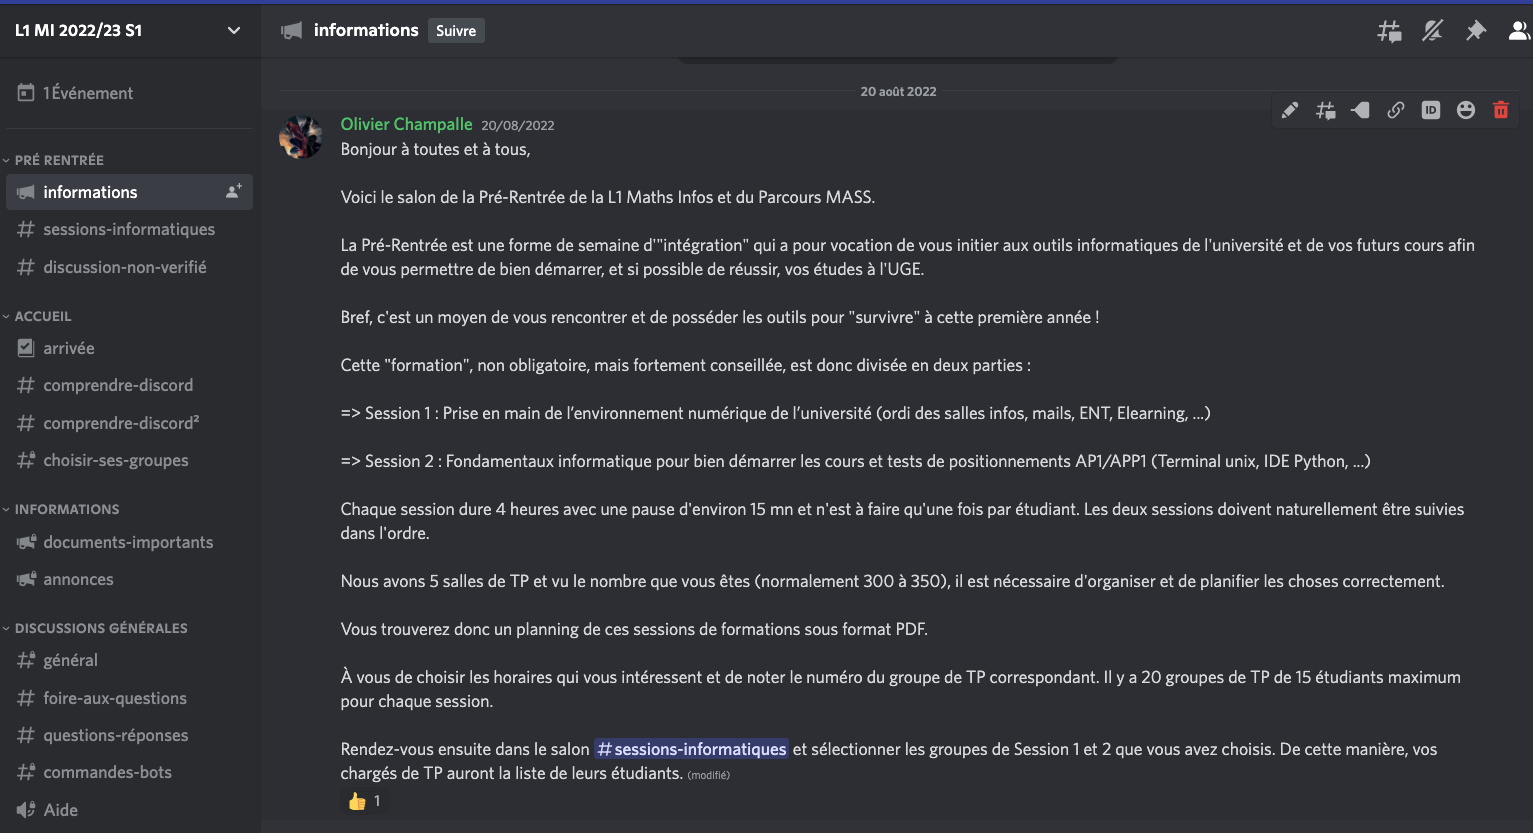
\includegraphics[scale=0.3]{Apercu_Discord_L1.png}
    \caption{Aper\c cu du discord de la L1}
     \end{center}
\end{figure}  

Par défaut et ce jusqu'au 1er octobre 2022, tous les nouveaux arrivants ont le rôle ``étudiant''. Ce qui veut dire que vous voyez apparaître et avez accès à toutes les catégories du discord réservées au rôle ``étudiant''. Au delà du 1er octobre 2022 vous serez obligé de vous faire valider ! La procédure de validation est clairement expliquée dans la catégorie ``Accueil''. A partir du 1er octobre 2022, si vous n'avez pas de numéro étudiant, cela sera juste impossible !

En parlant de la catégorie ``Accueil'', c'est clairement le premier endroit où cliquer ! Donc allez dans la catégorie ``Accueil'' et dans le salon ``arrivée''. Vous verrez apparaître un petit guide de formation sur discord et les bonnes pratiques à respecter, notamment se \textbf{renommer} ! Il y a pas mal d'informations à lire donc prenez votre temps.

Dans la catégorie de la ``Pré Rentree'', vous devriez aussi voir apparaître deux groupes vous concernant \\
``Session\_1\_GrX'' et ``Session\_2\_GrY'' , X et Y correspondant respectivement au groupe de la Session\_1 et de la Session\_2 que vous avez choisi dans le salon ``sessions-informatiques'' de la catégorie ``Pré Rentree''.

Ces salons respectifs vous permettront de communiquer avec vos chargés de TP respectifs, vos collègues de TP, de partager et d'accéder à des documents, notamment les sujets des sessions 1 et 2.

\end{exercice}

\section {Services en ligne}

Nous allons maintenant faire un tour des principaux services en ligne qui sont
mis à votre disposition à l'université, en particulier l'ENT (abréviation de
\emph{Environnement Numérique de Travail}) qui rassemble plusieurs services qui vous
seront utiles au cours de votre vie étudiante. 
 
\begin{exercice}[Environnement Numérique de Travail (ENT)]

\textbf{Attention: } Si vous vous êtes loggé avec un compte temporaire, cet exercice pourrait poser quelques difficultés d'accès à certaines applications, réservées aux ``login'' étudiants validés.
Si vous êtes dans ce cas là, vous suivrez avec un voisin et/ou avec votre chargé d'enseignement (si il peut partager son écran d'une manière ou d'une autre). Vous pourrez le refaire chez vous avec vos identifiants définitifs.

\begin{enumerate}
\item Avec votre navigateur web (par exemple Firefox), accédez à l'adresse \url{https://ent.univ-eiffel.fr}.
\item Vous découvrez l'écran d'accueil de votre Environnement Numérique de Travail comportant plusieurs ``rubriques'' représentant des applications que vous ``pourriez'' utiliser tout au long de votre scolarité.

\begin{figure}[h!]
    \begin{center}
    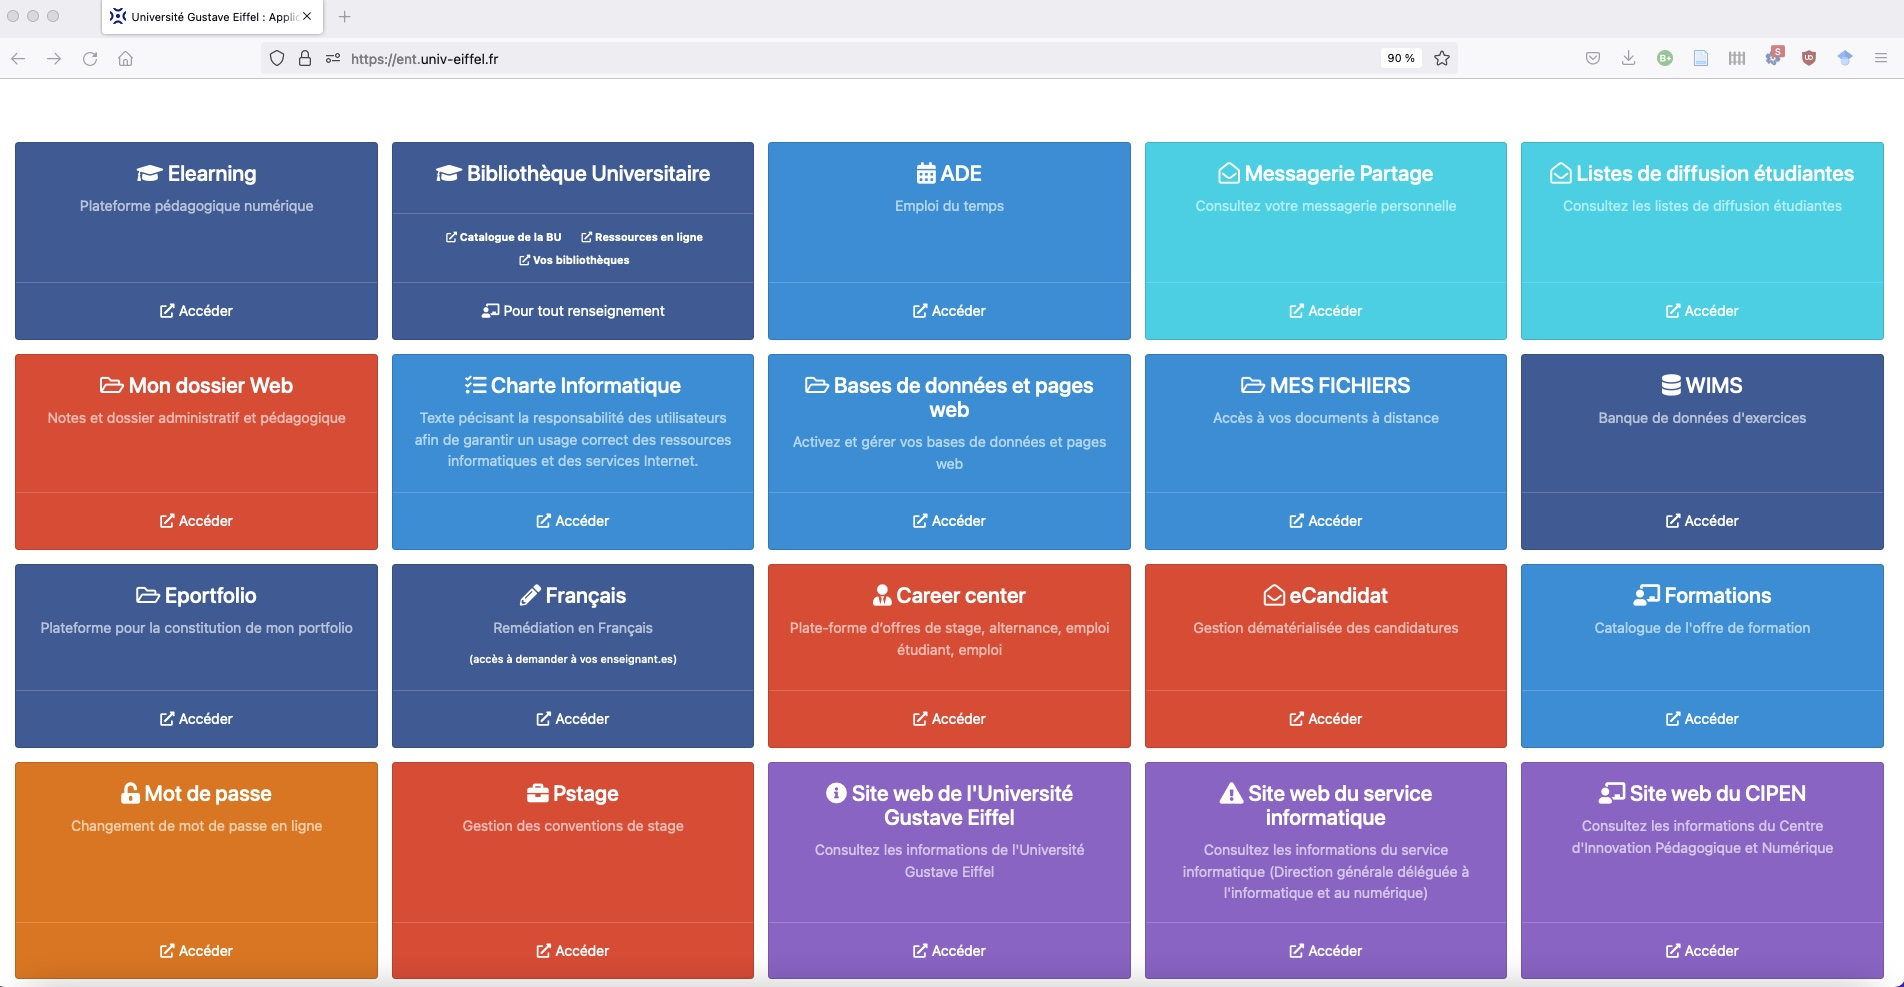
\includegraphics[scale=0.25]{ENT.jpg}
     \caption{Environnement Numérique de Travail}
     \end{center}
\end{figure}    

\end{enumerate}

\end{exercice}

\begin{exercice}[Annuaire]

Un annuaire contenant les coordonnées des enseignants et personnels de l'UGE est disponible tout en bas du site web de l'UGE
 \url{https://www.univ-gustave-eiffel.fr/}. Cette page est aussi accessible via l'icône suivante (en bas de l'ENT ):

\begin{figure}[h!]
    \begin{center}
    \includegraphics[scale=0.2]{siteWebUGE.jpg}
    \caption{Accès au site web de l'UGE via l'ENT}
     \end{center}
\end{figure}    

Il est également possible d'y accéder directement à l'adresse
\url{https://pagespro.univ-gustave-eiffel.fr/}, ou à l'aide d'une requête Google (par exemple, \emph{ annuaire Eiffel}). Ce n'est pas réellement un service mis à disposition uniquement pour les étudiants mais c'est utile quand même !

\begin{enumerate}
\item Vérifiez que vous connaissez bien les noms et prénoms de vos responsables de formation et/ou de 
cours pour cette première année. Par exemple : 
  \begin{enumerate}
  	\item Responsable de la L1 Maths-Info : M. Francis RIBAUD
  	\item Gestionnaire administrative de la L1 : Mme Ramatoulaye BARRY   
  	\item AP1 : M. Antoine MEYER et Mme Marie VAN DEN BOGAARD
  	\item APP1 : M. Wenjie FANG
  	\item Responsable Parcours MIASHS : M. Thierry BERKOVER et M. Pierre-André ZITT
   \end{enumerate}     
\item Recherchez sur l'annuaire du personnel leur numéro de bureau, de téléphone ainsi que leur adresse électronique.
\item Enregistrez ces informations dans un fichier texte nommé \texttt{``contacts.txt''} que
   vous stockerez dans le répertoire ``preRentree'' (autre part que sur le bureau donc ...)
\end{enumerate} 

 \textbf{Remarque: }Tous les enseignants ne sont pas toujours des personnels de l'Université,  
  ils n'apparaissent donc pas tous dans l'annuaire.\\
  Certains enseignants ne font pas apparaître leurs coordonnées complètes sous l'annuaire .... \c ca arrive aussi.
 
\end{exercice}

\begin{exercice}[Messagerie électronique personnelle (email)]

Ici nous allons parler d'un élément particulièrement essentiel, à savoir votre \textbf{Messagerie Partage}
(une rubrique bleu clair avec un petit message). La messagerie personnelle est réellement \underline{importante}.
C'est via cette messagerie que vous serez contacté par et que vous contacterez l'administration ainsi que vos enseignants. 
Les messages peuvent être réguliers pensez à la regarder régulièrement. 
Accéder à votre messagerie se fera en deux temps : 
\begin{enumerate}
\item Cliquez sur l'icône de la figure 4

\begin{figure}[h!]
    \begin{center}
    
\includegraphics[scale=0.25]{messagerie.jpg}
    \caption{Messagerie partage}
     \end{center}
\end{figure}    

\item Connectez-vous au service d'authentification de l'université (figure 5)

\begin{figure}[h!]
    \begin{center}
    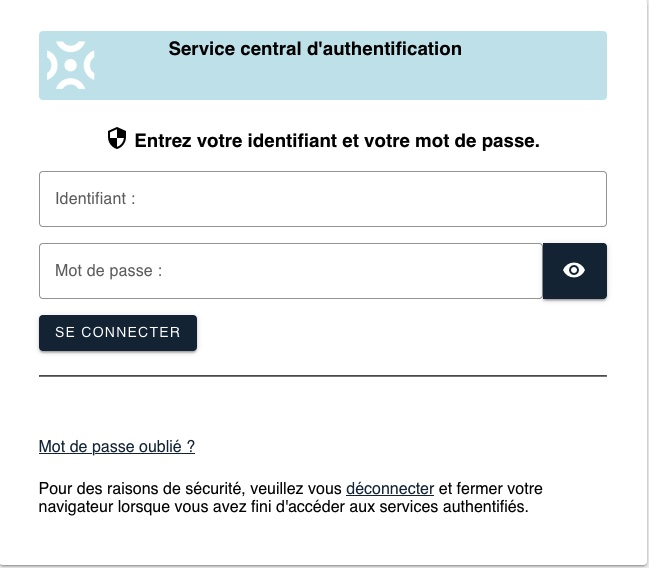
\includegraphics[scale=0.23]{authentification.jpg}
    \caption{Service d'authentification de l'université}
     \end{center}
\end{figure}    

\item Accédez ensuite à votre webmail (figure 6)

\medskip

Prenez le temps de découvrir les différentes fonctionnalités de cette interface. Normalement vous êtes assez familier de ce genre de webmail cela ne devrait pas trop vous perturber.

\begin{figure}[h!]
    \begin{center}
    \includegraphics[scale=0.25]{mail.jpg}
    \caption{Aper\c cu de la fenêtre du webmail}
     \end{center}
\end{figure}    
\end{enumerate}
%\newpage

A présent, histoire de vous faire la main, vous allez tout simplement envoyer un mail à votre chargé de TP qui vous donnera gentiment son adresse mail :-). 

Suivez la procédure suivante : 

\begin{enumerate}
\item Sur la page de votre messagerie,  cliquez sur \textbf{Nouveau message} ou appuyez
   sur la touche \texttt{N}.  Pour utiliser le raccourci clavier,   veillez à ne pas déjà
   avoir cliqué dans un champ de texte.
   \begin{itemize}
   \item \textbf{A} contient l'adresse du ou des destinataire(s) de votre email.
   \item \textbf{CC} permet d'envoyer une Copie Conforme de votre email à des
      destinataires supplémentaires. Ceux-ci sauront que l'email ne leur est
      pas adressé directement mais les concerne (par exemple,   pour envoyer à
      votre binôme une copie d'un message destiné à un enseignant).
   \item \textbf{CCI} permet d'envoyer une Copie Conforme Invisible (en anglais \emph{Blind
      Carbon Copy}) de votre email à des destinataires sans que les autres
      destinataires du courrier ne le voient.
   \item \textbf{Sujet} contient le \emph{titre} de votre email.
   \end{itemize}
   
\item Sur votre webmail,   remplissez les champs comme indiqué ci-dessus afin
   d'envoyer un email à votre chargé de TP dont le sujet doit être : ``L1 -
   présentation de \emph{nom}  \emph{prénom}'',   où \emph{nom} sera remplacé par votre nom de famille et \emph{prénom} par votre prénom.
   
\item Dans le corps du message,  copiez/collez le contenu du fichier \texttt{``presentationNomPrenom.txt''}.
   N'oubliez pas d'ajouter à votre message un \emph{Bonjour} et une formule de politesse :
   vous obtiendrez certainement plus facilement ce que vous demandez !
   Envoyez votre mail de présentation en cliquant sur \textbf{Envoyer} ou
   en appuyant sur \texttt{ctrl + Entrée}.

\medskip

   \textbf{Attention ! : } Même si vous disposez d’une adresse email personnelle,   il
   est \textbf{impératif} que vous consultiez régulièrement votre compte de
   messagerie à l’université. Des messages importants concernant le déroulement
   des cours vous y seront régulièrement envoyés.

\item (Bonus) Si vous le souhaitez, il est possible de rediriger votre courrier
   vers une adresse extérieure. 

\medskip

   Pour recevoir vos emails étudiants sur votre adresse habituelle,   cliquez sur
   l'onglet \textbf{Préférences},   allez dans la partie \textbf{Mail},   cherchez la section
   \textbf{Réception des mails} (figure 7) puis renseignez votre adresse dans le champ \textbf{Faire
   suivre une copie à}. \\
   Configurez alors votre système d'email habituel afin
   de pouvoir envoyer des emails depuis celui-ci en utilisant votre identité
   étudiante \texttt{login@etud.univ-eiffel.fr} comme expéditeur.
 
 \begin{figure}[h!]
    \begin{center}
    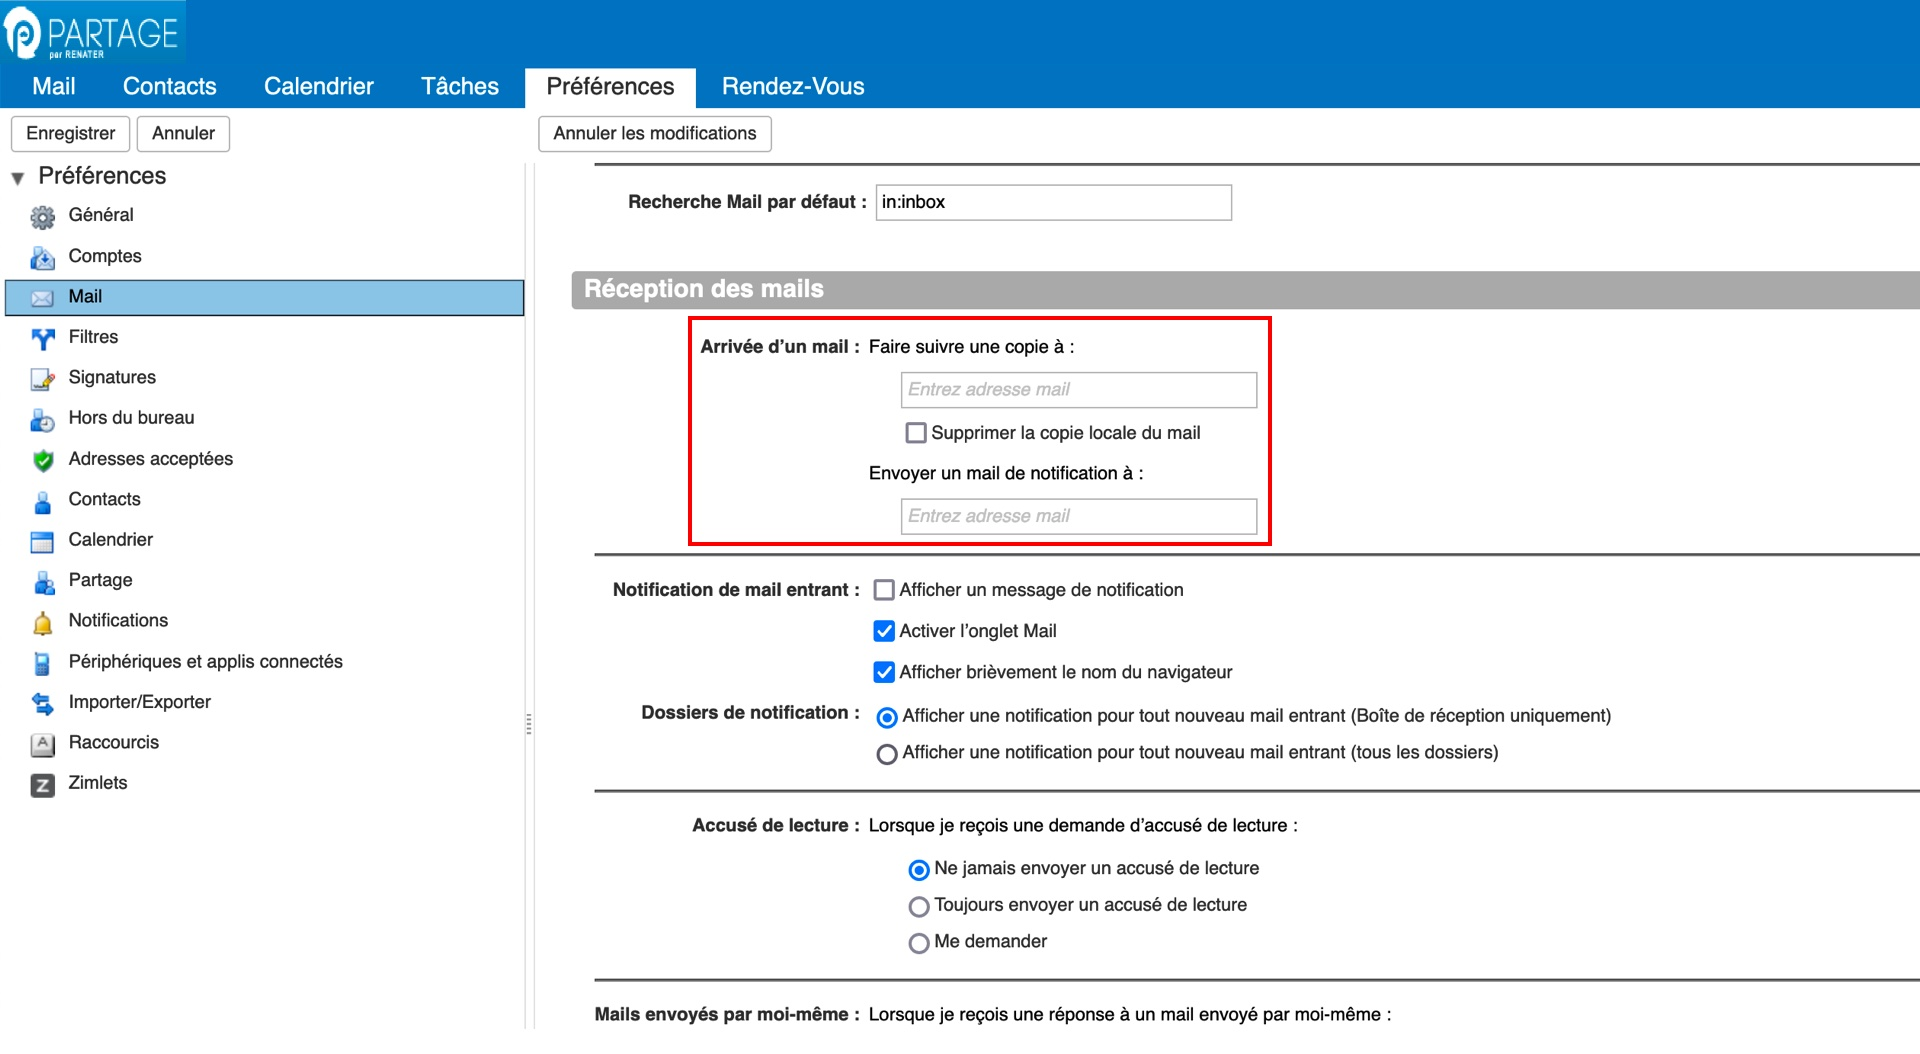
\includegraphics[scale=0.25]{copie_mail.jpg}
    \caption{Configuration de suivi des mails}
     \end{center}
\end{figure}    

\item (Bonus bis) Accès au service de messagerie via un client mail (protocoles IMAP/SMTP) pour celles et ceux qui connaissent \url{https://cri.u-pem.fr/service-aux-etudiants/messagerie} 

\end{enumerate}

%\newpage

\end{exercice}

\begin{exercice}[Accès à vos fichiers depuis un navigateur]

\begin{enumerate}
\item Il est également possible de visualiser le contenu de votre répertoire
    personnel directement sur l'ENT (à condition d'avoir un compte). Pour cela,  cliquez sur la rubrique \textbf{Mes fichiers} (figure 8).

\begin{figure}[h!]
    \begin{center}
    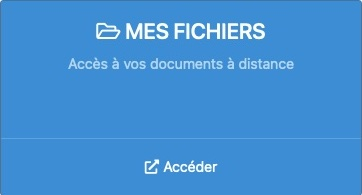
\includegraphics[scale=0.25]{mesFichiers.jpg}
    \caption{Accès à vos documents à distance}
     \end{center}
\end{figure}    
        
\item Utilisez cette fonctionnalité pour chercher les fichiers créés
    précédemment (cliquez dans l'arborescence figure 9).
    
 \begin{figure}[h!]
    \begin{center}
    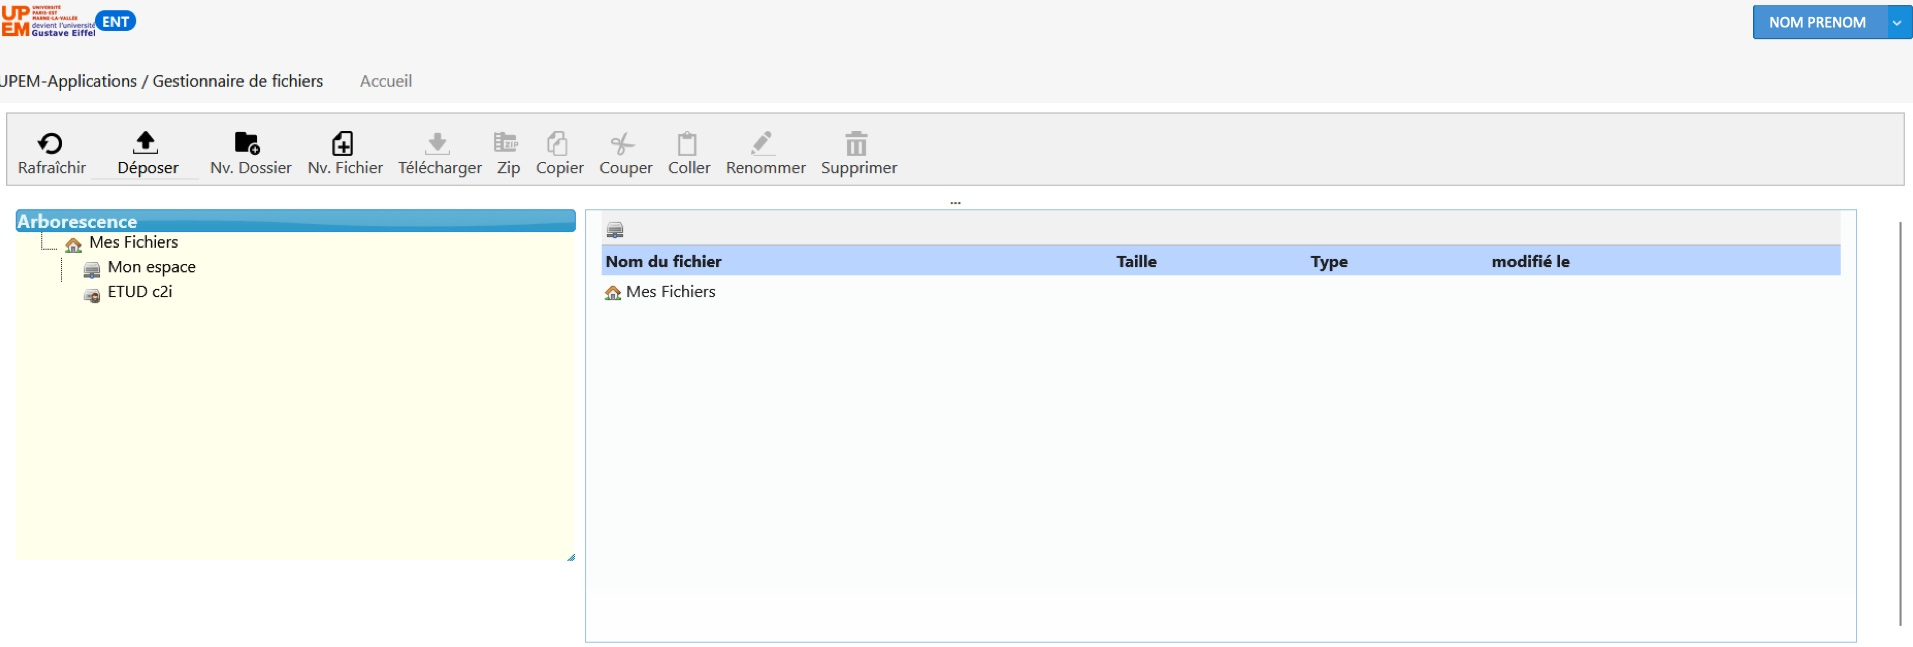
\includegraphics[scale=0.25]{AccesMesFichiers.jpg}
    \caption{Interface d'accès au répertoire personnel}
     \end{center}
\end{figure}    

\item Faites le tour des fonctionnalités présentes : création de nouveau dossier, de nouveau fichier, ...  

\item Essayer de télécharger un fichier dans un répertoire (il suffit de cliquer dessus, c'est automatique)

\item Un bouton droit de la souris sur les dossiers et les fichiers dans la partie droite vous permettra de télécharger sous format ZIP, de copier, de couper, de renommer ou de supprimer (figure 10).

\begin{figure}[h!]
    \begin{center}
    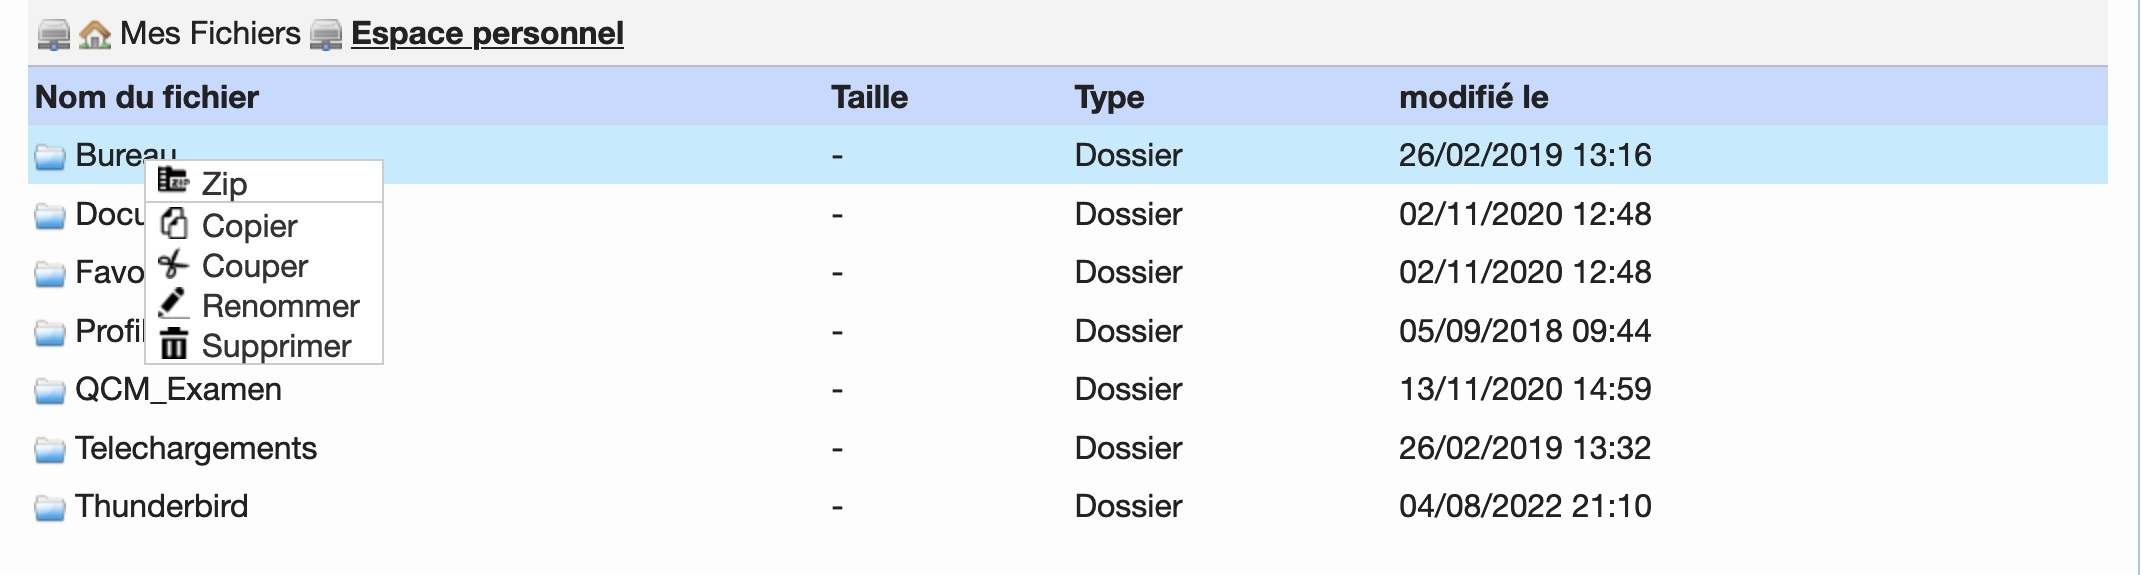
\includegraphics[scale=0.2]{mesFichiersMenu.jpg}
    \caption{Menu contextualisé}
     \end{center}
\end{figure}    
      
\end{enumerate}

\textbf{Note 1: } Grâce à cette fonctionnalité,   vous pouvez récupérer vos fichiers
sans être physiquement à l'université.

\medskip

\textbf{Note 2: } Il existe \underline{un quota maximum de stockage} que vous ne pouvez pas dépasser : environ 2 gigas ! Donc soyez vigilant sur la taille de vos données, vous pourriez le regretter.

\medskip

\textbf{Au fait, au fait ! } Si vous êtes observateur(trice) vous avez peut être constaté que l'icône en haut à gauche de la figure 9 est différente de celle de l'université Gustave Eiffel (voir figure 11)

\begin{figure}[h!]
    \begin{center}
    
\includegraphics[scale=0.2]{UGEvsUPEM.jpg}
    \caption{Différence entre logo UGE et U-PEM}
     \end{center}
\end{figure}    

C'est .... presque normal ! En fait l'application d'accès à distance à votre répertoire personnel est lié à un ancien ENT. \c Ca marche bien mais si vous cliquez sur le menu ``Accueil'' vous serez conduit sur l'ancien ENT auquel vous n'avez pas accès comme le montre la figure 12 ! 

\begin{figure}[h!]
    \begin{center}
    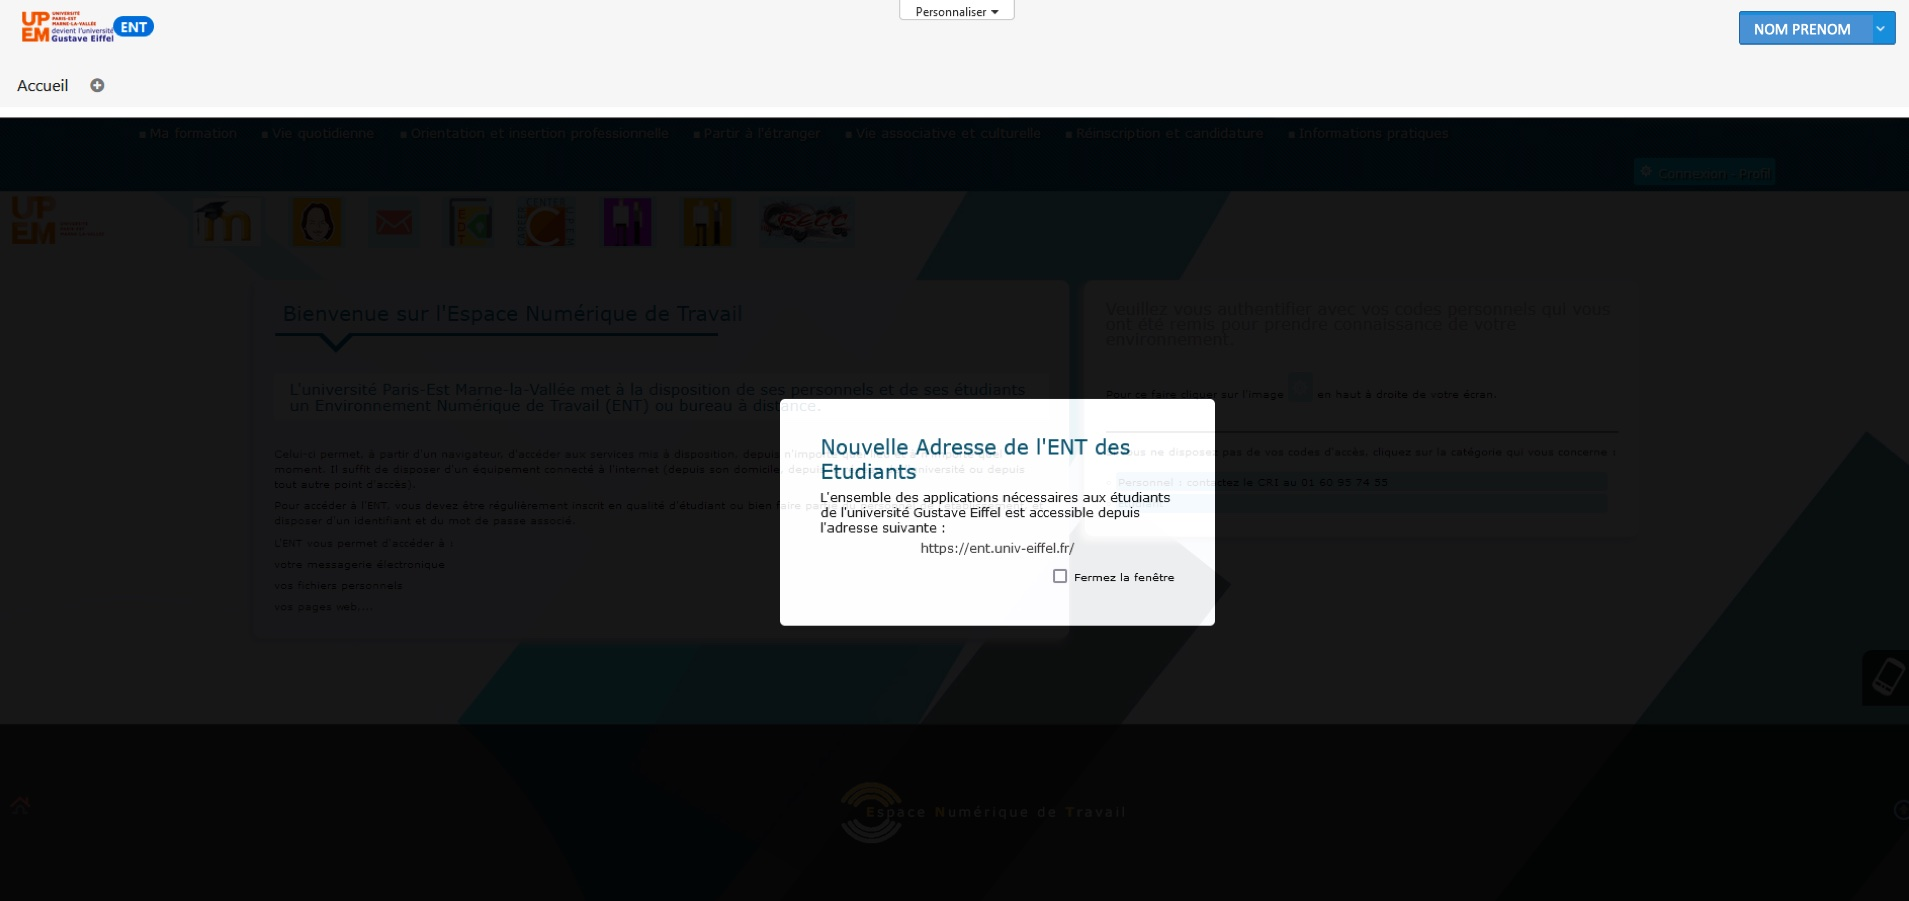
\includegraphics[scale=0.25]{MesFichiersAccueil.jpg}
    \caption{Accès non autorisé à l'ancien ENT}
     \end{center}
\end{figure}    

Du coup, pas de panique, il faudra revenir sur l'adresse : \url{https://ent.univ-eiffel.fr}. C'est un ``problème'' à prendre en compte et qui pourrait aussi apparaître sur d'autres applications de l'ENT.

\newpage

\end{exercice}

\begin{exercice}[Moodle : plateforme d'enseignement à distance]

La plateforme Moodle (aussi appelée Elearning) est accessible depuis votre ENT
(icône avec un chapeau de diplômé). Accédez-y.

\begin{figure}[h!]
    \begin{center}
    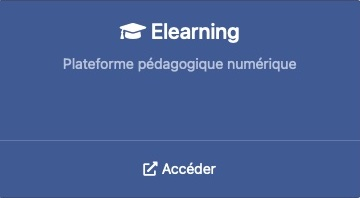
\includegraphics[scale=0.25]{iconeElearning.jpg}
    \caption{Accès au Elearning}
     \end{center}
\end{figure}    

\medskip

\textbf{Note 1 : } Les noms \emph{Moodle} et \emph{Elearning} seront utilisés de manière
interchangeable par vos enseignants.

\medskip

\textbf{Note 2 :} Il est aussi possible d'accèder directement au Moodle de l'UGE via l'URL
\url{http://elearning.univ-eiffel.fr}.

\medskip

Elearning est une plateforme de cours en ligne (basée sur la plateforme Moodle),  qui permet de consulter des
fichiers mis à disposition par les enseignants,  des cours, des sujets de TD, de TP et des
annonces. Elle permet aussi de déposer vos propres fichiers afin de les
soumettre pour évaluation (rendre un TP ou un projet par exemple).

Comme pour chaque première connexion au Elearning, il faudra tout d'abord vous logger au moins une première fois. 
Cliquer en haut à droite de la page d'accueil (que vous pouvez prendre le temps de visiter d'ailleurs).

\begin{figure}[h!]
    \begin{center}
    \includegraphics[scale=0.13]{ElearningAccueil.jpg}
    \caption{Page d'accueil du Elearning}
     \end{center}
\end{figure}    

Bienvenue sur votre tableau de bord personnel (figure 14)! C'est ici que vous verrez apparaître tous vos cours dans la partie ``VUE D'ENSEMBLE DES COURS''.
Un cours n'apparaît que si vous y êtes inscrit.\\
L'inscription à un cours se fait par l'enseignant responsable du cours et/ou les intervenants possédant les droits nécessaires.
Normalement l'inscription est automatique pour tout étudiant possédant une adresse mail UGE valide.

\newpage

Prenez à nouveau le temps de découvrir cette page avec votre chargé de TP, maintenant que vous êtes loggé, il y a plus de fonctionnalités qui apparaissent :

\begin{enumerate}
\item Sur la gauche de la page plusieurs icônes ont fait leur apparition
\item Sur la droite, une flèche blanche sur fond bleu fera apparaître une fenêtre glissante avec un rappel de vos évènements à venir et vos messages
\item En bas de la page plusieurs nouvelles informations telles les derniers éléments consultés, une to-do-liste, ... 
\end{enumerate}

\textbf{Note :} Moodle est un outil très puissant possédant moult fonctionnalités qui ne sont pas toujours utilisées par les enseignants et qui ne sont pas toujours faciles à comprendre non plus.

\medskip

À présent dans la partie ``VUE D'ENSEMBLE DES COURS'' vous devriez voir apparaître le cours suivant : 

\begin{figure}[h!]
    \begin{center}
    
\includegraphics[scale=0.3]{Logo_2023-24.png}
    \caption{Cours de pré-rentrée}
     \end{center}
\end{figure}    

Si vous ne voyez pas le cours c'est que vous n'êtes pas inscrit, votre chargé de TP va s'en occuper (uniquement si vous avez une adresse UGE bien sûr !). Ce sera l'occasion pour vous de voir comment il/elle fait.

\medskip

Une fois inscrit au cours, vous voyez un premier cadre gris : ``Bienvenue dans le cours de pré-rentrée 2022-23''. Vous y trouverez une première chose à faire : choisir votre groupe de TP de pré-rentrée !
C'est une action obligatoire pour avoir le droit d'accès au contenu du cours. \\
Naturellement tous les cours ne sont pas con\c cus de la même manière, mais pour aujourd'hui ce système est très pratique notamment pour que votre chargé de TP puisse vous envoyer, uniquement à votre groupe, un message de bienvenue via le forum des nouvelles.

\medskip

Le forum des nouvelles permet aux enseignants d'envoyer des messages à l'ensemble ou à un groupe spécifique d'étudiants. Dans le cadre de ce cours, dès qu'un message est envoyé, les étudiants re\c coivent une copie par mail. \\
Vérifiez que vous avez bien re\c cu un message mail et que vous accédez bien au message de votre chargé de TP !
 
\medskip

Maintenant parlons de la section ``Session 1 : Prise en main de l’environnement numérique de l’université'' que vous voyez apparaître.\\
Dans cette section, vous allez trouver le sujet du TP de la session 1 (que vous êtes déjà en train de lire). Ouvrez le en cliquant dessus !   

Localisez aussi la ``zone de rendu de la session 1'' et suivez les consignes qu'elle contient.

\end{exercice}

\begin{exercice}[Centre de Ressource Informatique]
Le Centre de Ressources Informatique (C.R.I.) est le service de l'Université qui permet :

\begin{itemize}
\item d'assurer le développement cohérent des moyens informatiques,   réseaux,   et des systèmes
d’information de l'Université ;

\medskip

\item de garantir la disponibilité des ressources informatiques et la sécurité des réseaux 
sur l'ensemble de l'Université.
\end{itemize}

Il est situé au 4ième étage, bureau 4B211, du batiment Copernic. Hotline : 01 60 95 74 55.

\medskip

En cas de difficultés avec les outils présentés plus haut, ce seront vos meilleurs amis !

\medskip

Vous pouvez accéder à leur service directement par un lien sous l'ENT : 

\begin{figure}[h!]
    \begin{center}
    \includegraphics[scale=0.25]{CRI_ENT.jpg}
    \caption{Centre de Ressource Informatique sous l'ENT}
     \end{center}
\end{figure}    

La page web \url{https://cri.u-pem.fr/service-aux-etudiants/faq}
présente un certain nombre de problèmes souvent rencontrés et des solutions simples à mettre
en œuvre pour les résoudre. Ces problèmes récurrents pourraient être :
\begin{itemize}
\item \emph{J'ai effacé par erreur un fichier sur mon compte,   peut-on le récupérer?}

\item \emph{J'ai perdu mes identifiants ?}
\end{itemize}

\end{exercice}

\begin{exercice}[Le reste des applications de l'ENT en vrac]

%Dans cette section sont présentées en ``vrac'' le reste des applications de l'ENT auxquelles vous pourriez avoir accès.

\begin{figure}[h!]
    \begin{center}
    
\includegraphics[scale=0.25]{EntEnVrac12.png}
    \caption{ENT reste des applications en vrac (1/4)}
     \end{center}
\end{figure}    

\begin{figure}[h!]
    \begin{center}
    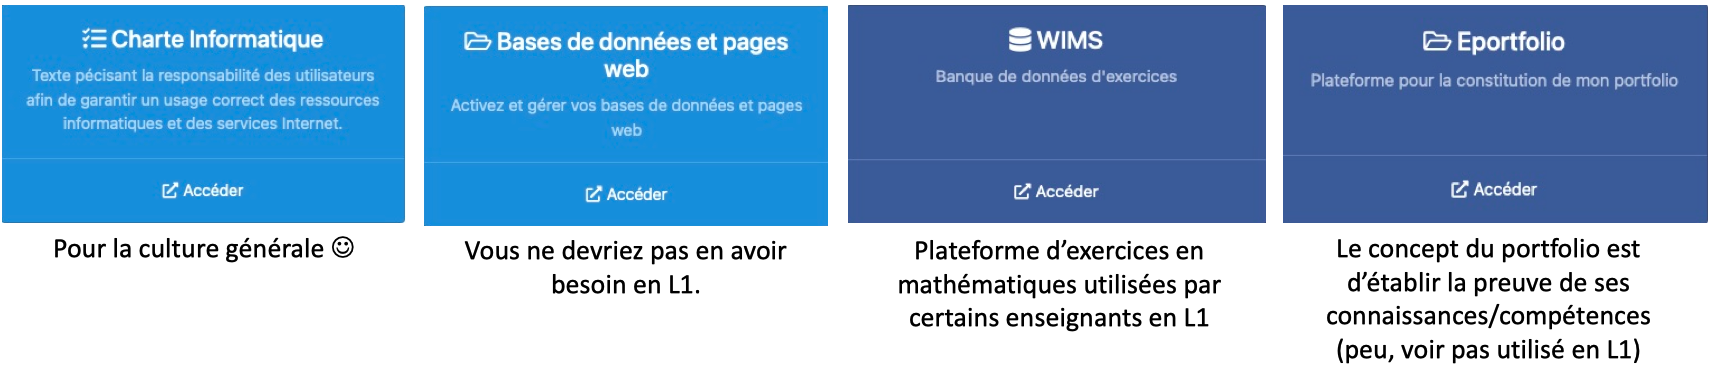
\includegraphics[scale=0.25]{EntEnVrac21.png}
    \caption{ENT reste des applications en vrac suite (2/4)}
     \end{center}
\end{figure}    

\begin{figure}[h!]
    \begin{center}
    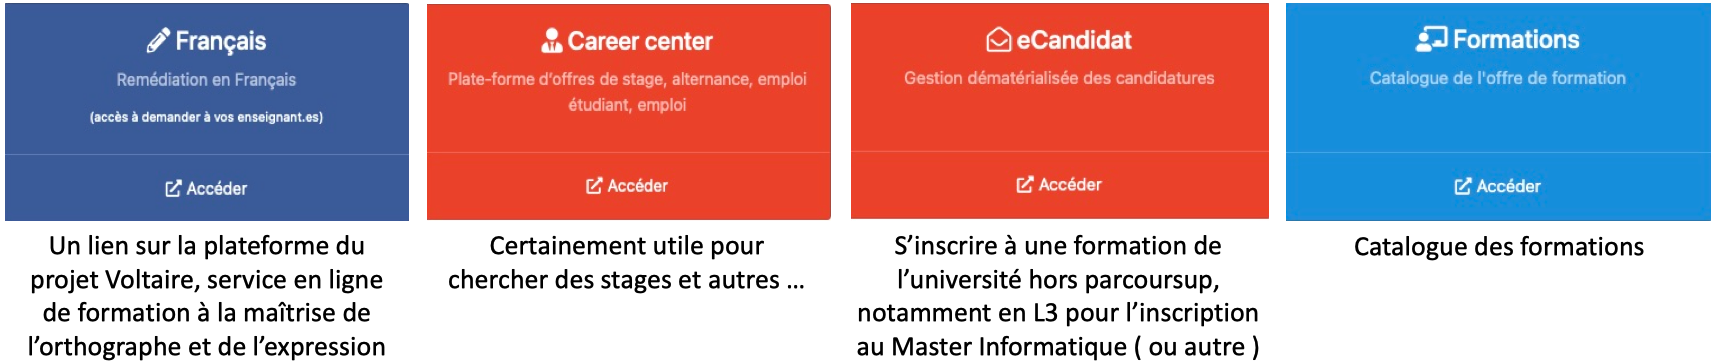
\includegraphics[scale=0.25]{EntEnVrac31.png}
    \caption{ENT reste des applications en vrac suite (3/4)}
     \end{center}
\end{figure}    

\begin{figure}[h!]
    \begin{center}
    \includegraphics[scale=0.22]{EntEnVrac2.jpg}
    \caption{ENT reste des applications en vrac suite et fin (4/4)}
     \end{center}
\end{figure}    

\end{exercice}

\newpage

\section{Python et Notebook Jupyter}

Pour les L1 Maths-Infos en particulier, vous serez confrontés à l'utilisation de fichier très particulier. Il s'agit de fichier ``Notebook Jupyter''. Tous vos cours de Python seront sous ce format là,
il est donc important de savoir les manipuler un peu.

La solution Jupyter Notebook est une application web open source qui permet de créer et de partager des documents contenant du code en direct, des équations, des visualisations et du texte narratif. 

Le plus souvent, Jupyter Notebook est utilisé dans un environnement Python. Ils ont des sorties très interactives et peuvent être facilement partageables, tout comme un cahier ordinaire.

Il y a deux fa\c cons de procéder pour exploiter les cours au format Jupyter : 

\begin{enumerate}
\item à distance via l'application Binder (session 1)
\item en téléchargeant les fichiers et en les ouvrant directement sur votre machine (session 2)
\end{enumerate}

Nous allons voir la première méthode au cours de cette session 1. Vous découvrirez les fameuses particularités de ces notebooks !\\
La deuxième méthode sera vue lors de la session 2.

\newpage

\begin{exercice}[Notebook, avec myBinder]

Nous allons apprendre à ouvrir ce type de fichier de manière distante grâce
à l'outil en ligne \textbf{myBinder}. Il vous permettra de consulter le cours de chez vous, voire
même dans le bus ou le rer sur votre téléphone !

Aller sur le Elearning, dans la section de la session 1 
Vous y trouverez un lien sur le cours. Cliquez sur ce lien et laisser faire les choses.
Une nouvelle fenêtre s'ouvre dans le navigateur et vous emmène sur la page de la (figure 21). A vous de cliquez sur le lien de la figure 22. 

\begin{figure}[h!]
    \begin{center}
    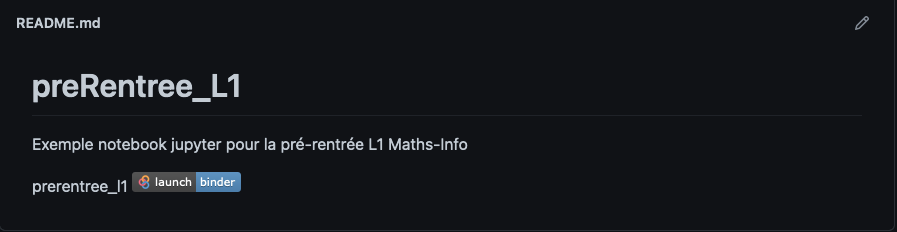
\includegraphics[scale=0.35]{Github_MyBinder.png}
    \caption{Première page d'accès au cours à partir du site GitHub}
     \end{center}
\end{figure} 

Cliquez sur le lien ``launch\_Binder''. Attention cela pourrait prendre un peu de temps de chargement.
Vous devriez voir apparaître la figure 22.

\begin{figure}[h!]
    \begin{center}
    \includegraphics[scale=0.35]{jupytermyBinder.png}
    \caption{Environnement jupyter avec myBinder}
     \end{center}
\end{figure}    

Une nouvelle page web vient de s'ouvrir. Vous avez ouvert votre premier document jupyter. \\
Chaque rectangle gris s'appelle une cellule Python. Par défaut,   elles sont
    toutes évaluées. Pour supprimer cela,   cliquez sur \texttt{kernel} puis 
    \texttt{restart \& clear outputs}.
    
Placer le curseur sur la première cellule,   puis tapez \texttt{Shift + Entrée} : vous allez
    évaluer votre première cellule. Le notebook devrait afficher \texttt{6} en bleu juste en dessous
    de la cellule.
    
Vous pouvez facilement modifier le contenu d'une cellule. Remettez le curseur sur
    la première cellule (il devrait être arrivé sur la seconde cellule),   sélectionner \texttt{6} et
    remplacez le par \texttt{10}. Vous pouvez alors re-évaluer la cellule.

\textbf{Note :}  une vidéo de démonstration est aussi disponible dans la section de la session 1.

Notez, néanmoins, que toutes vos modifications sur ce document ne pourront pas être enregistrées. C'est normal c'est un document d'entraînement.\\
Vous avez maintenant le kit de survie pour lire, travailler et apprendre les cours de Python. 

\end{exercice}

\section{Besoins informatiques divers}

A présent que vous avez un bon aper\c cu de l'environnement informatique de l'UGE et des applications qui vous seront nécessaires pour ``survivre'' a minima à la L1, il est temps de faire le point sur vos moyens informatique personnel ! 

\subsection{Ordinateur personnel}

En premier lieu avez-vous un ordinateur personnel (fixe ou portable) pour travailler chez-vous ? Si ce n'est pas le cas, vous pouvez vous signaler auprès de votre chargé de TP qui remontera l'information à l'administration de la L1. Vous pourriez ainsi peut être bénéficier d'un programme d'assistance aux personnes en détresse numérique. Donc n'hésitez pas (mais ne trichez pas) !

%Ensuite, si vous avez un ordinateur ``suffisamment'' correct (RAM et ROM), la question est : vous sentez vous capable d'installer une version Debian sur votre PC genre en dual boot (demandez à vos chargés de TP pour les termes techniques). Si ce n'est pas le cas sachez qu'il y a deux solutions possibles : \\
%
%\begin{itemize}
%\item
%Une machine virtuelle installable sous tout OS 
%\item
%WSL : Windows Subsystem for Linux
%\end{itemize}
%
%\subsection{Machine virtuelle}
%
%Pour celles et ceux qui ont apporté leur ordinateur personnel, et qui ont pris beaucoup d'avance, votre chargé de TP peut vous aider à installer une machine virtuelle Debian pour ``émuler'' le comportement d'un ordinateur avec un Os Debian.\\
%Sous le Elearning rendez-vous dans la section de la session 1 et cliquez sur le lien Machine Virtuelle : ``Utiliser debian via VirtualBox sur votre ordinateur personnel'' et laisser vous guider.
%
%Attention, cela prend du temps, donc mieux vaut faire \c ca chez-vous ! Cette VM n'est pas non plus une solution parfaite mais elle vous permettra de progresser.
%
%Vous trouverez trois vidéos faites pour vous aider : 
%
%\begin{itemize}
%\item
%Tuto Vidéo - 1. Installation de VirtualBox
%\item
%Tuto Vidéo - 2. Mise à jour de la VM
%\item
%Tuto Vidéo - 3. Configuration extension
%\end{itemize}
%
%\subsection{WSL : Windows Subsystem for Linux}
%
%Comme son nom l'indique WSL est un service principalement dédié au OS Windows. Il permet d'émuler en mode terminal le comportement d'un OS de type LINUX. 
%Seule les version 10 et 11 de Windows sont concernées. 
%Là encore un guide vous est offert sur Elearning. Néanmoins internet reste aussi votre meilleur ami.

\subsection{Configuration du WIFI avec Eduroam}

L'Université Gustave Eiffel possède un réseau WIFI accessible aux étudiants : Eduroam. Il s'agit d'un réseau sécurisé et déployé en Europe qui est accessible dans la plupart des universités françaises avec les mêmes identifiants. 

La procédure de connexion est disponible ici : \url{https://cri.u-pem.fr/documentation/comment-configurer-le-wifi}

\section {Place au test de parcours et de positionnement AP1/APP1}

Lors de la réunion de pré-rentrée organisée par le responsable de la L1, Francis RIBAUD, il vous a été expliqué qu'il existait deux modules d'Algorithmique et de Programmation en parallèle : AP1 et APP1. 

\begin{itemize}
\item 
\textbf{AP1} est fait pour les personnes qui débutent en informatique et en particulier en langage Python. Les cours sont organisés de manière assez classique : cours magistraux, travaux dirigés et séances de travaux pratiques. La progression pédagogique est axée sur la découverte du langage Python à partir de la base.

\medskip

\item 
\textbf{APP1} est un module con\c cu pour les étudiants qui possèdent déjà un certain bagage en programmation (langage Python) et surtout en algorithmique. En général ce sont celles et ceux qui ont pris l'option NSI à partir de la 1ère et qui l'ont maintenue en Terminale mais pas que ! Toute personne motivée et possédant des bases en autodidacte sont les bienvenues aussi ! Ce module est principalement con\c cu sur la base de mini-projets, il n'y a pas de cours en soi \emph{(En soi est une locution adverbiale, qui signifie ``intrinsèquement, dans l’absolu'')}. Les étudiants d'APP1 peuvent cependant accéder aux cours d'AP1, notamment en amphi, mais leurs activités résident principalement dans la réalisation de projets en équipe.
\end{itemize}

Les places en APP1 sont limitées à 3 groupes de TP. Il a donc été décidé de permettre à chacune et à chacun de se positionner pour savoir dans quel module il/elle voudrait et pourrait aller. \\
D'où l'idée d'un test de positionnement. On parle bien de positionnement et pas d'évaluation ! Il ne s'agit en aucun cas d'un examen ! L'objectif n'est absolument pas de juger vos compétences, mais de vous aider à savoir si vos connaissances en algorithmique et en programmation python sont assez solides pour suivre le rythme pédagogique d'APP1.\\

Il y a deux questionnaires à faire sous Elearning (un seul questionnaire en version papier pour ceux/celles qui n'ont pas d'identifiants): 

\begin{itemize}
\item
``Votre parcours en informatique'', c'est un petit questionnaire pour mieux vous connaître : savoir qui vous êtes, d'où vous venez etc. Cool pas d'enjeux !
\item 
``Vos connaissances en Python et en algorithmique'', il s'agit du fameux test de positionnement AP1/APP1. Ce test concerne uniquement les personnes engagées en L1 Maths Infos (pas la filière MIASHS).
\end{itemize}

Les deux  tests de parcours et de positionnement dure environ 30-40 mn maximum cumulés sans trop se presser. Pour la version papier il s'agit d'un QCM que vous remettrez à votre chargé de TP (qui le remettra à d'autres personnes après). 

Faites ces tests de manière honnête, face à vous même, vous n'avez aucun intérêt à ``tricher'', ce qui compromettrait vos chances de réussite par la suite !

Bon courage et à bientôt !


\end{document}